\newcommand{\FIGSCALE}{0.68}

\section{Experimentation}
\label{sec:experimentation}

%To answer questions such as: what is the overhead of reaching
%consistent partitioning using \NAME in large scale networks and is
%\NAME relevant in Edge infrastructures where \processes are
%geo-distributed into clusters?
In this section, we discuss the evaluations of \NAME we conducted on top of
PeerSim, a simulator to
evaluate and assess distributed algorithms in large scale
networks~\cite{montresor2009peersim}. All the code is available % on % the
%Github platform
at \mbox{\url{https://github.com/ane-wane/as-cast}}.

%% \subsection{Confirm the complexity analysis stating that
%%   communication and time overheads depend on the current partitioning
%%   of the system.}

\subsection{Scalability and trade-off}
\begin{asparadesc}
\item [Objective:] Confirm the scalability of \NAME by highlighting the
  trade-off between the current partitioning of the system and the
  protocol's overhead in terms of generated traffic and termination
  time.
  
\item [Description:]
  
We build a network comprising 10k \processes. First, we chain
\processes together, then we add another link per
\process to another random \process. Since links are bidirectional,
each \process has 4 communication links on average. We set the latency
of links between 20 and 40 ms at random following a uniform
distribution.
%
To favor more concurrent operations, we % voluntary
set
weights and latency to different values: each link has a weight
between 5 and 15 set randomly using a uniform distribution. This
allows nodes to receive messages in different orders, % than their
% respective shortest path
therefore generating more messages to reach consistent
partitioning.


\noindent To evaluate dynamic consistent partitioning, we first
create 100 partitions one at a time: \processes reach consistent
partitioning before we create each new partition. Second, we remove
every partition one at a time, in the order of their creation, hence
starting from the first and oldest partition that had been added.

\noindent We measure the average number of messages % generated
per
\process per second; and the time before reaching consistent
partitioning after adding or removing a partition.


%% \begin{figure*}[t]
%%   \subfloat[\label{fig:complexity}Dynamic consistent partitioning overhead of \NAME.]{
%%     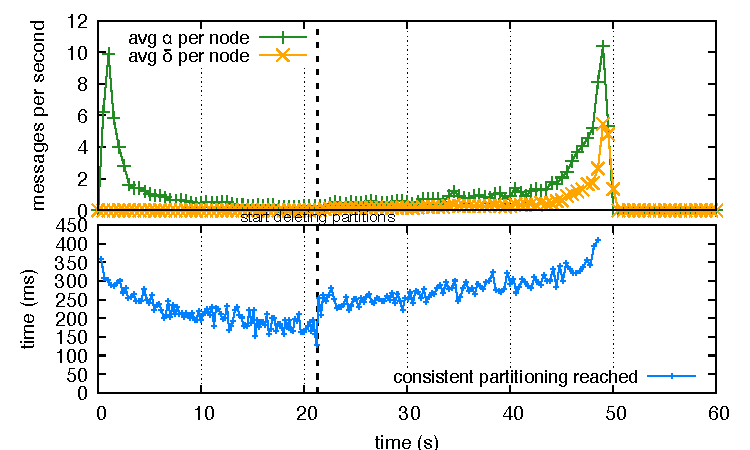
\includegraphics[width=\FIGSCALE\columnwidth]{img/as_cast_complexity.pdf} 
%%   }
%%   \hspace{5pt}
%%   \subfloat[\label{fig:geant}Partitioning overhead of 2
%%     clusters connected by a long distance link.]{
%%     \centering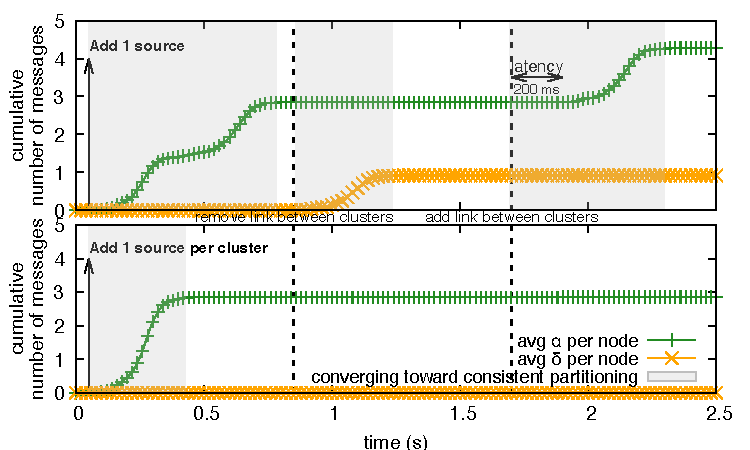
\includegraphics[width=\FIGSCALE\columnwidth]{img/as_cast_geant.pdf}
%%   }
%%   \caption{\TODO{\NAME overhead}.}
%% \end{figure*}

\begin{figure}[t]
  \centering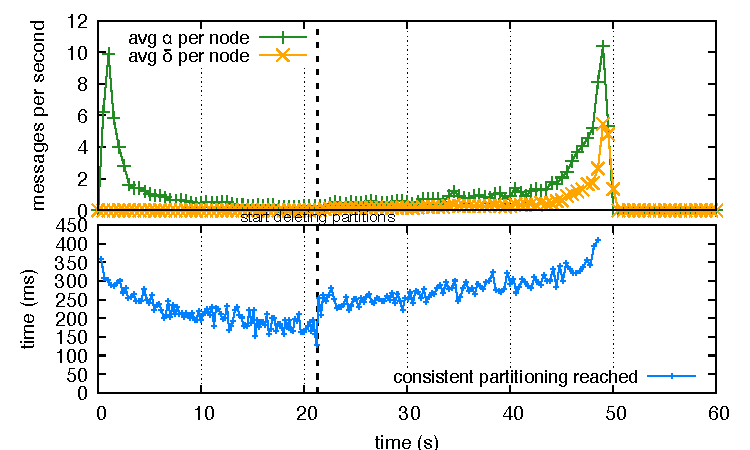
\includegraphics[width=\FIGSCALE\columnwidth]{img/as_cast_complexity.pdf}
  \caption{\label{fig:complexity}Dynamic consistent partitioning overhead of \NAME.}
  
%%   %% \caption{\label{fig:complexity}Cumulative average number of messages
%%   %%   per process in a network comprising 10k processes; along with the
%%   %%   duration before reaching consistent partitioning after adding or
%%   %%   removing a partition, totaling 100 new partition then removed.}
\end{figure}

\item [Results:]

Figure~\ref{fig:complexity} shows the results of this experiment. The
top part shows the average traffic per \process per second divided
between $\alpha$ and $\delta$ messages. The bottom part shows the time
before reaching consistent partitioning.

\noindent Figure~\ref{fig:complexity} confirms that \NAME's overhead
depends on the size of partitions. % In this scenario,
This % empirically
corresponds to a complexity in terms of number of messages of
$\mathcal{O}(\frac{|E|}{|V|\cdot|P|})$ where $E$ is the number of
links, $V$ is the number of \processes, and $P$ is the number of
partitions. In other terms, the $p^{th}$ partition contains $1/p$
\processes and reduces the size of closest partitions so every
partition has $1/p$ \processes on average.
  
\noindent Therefore, the first partition is the most expensive, for
$\alpha$ messages must reach every \process which takes time and
generate more traffic.  \NAME quickly converges towards consistent
partitioning in 350 milliseconds.
% TODO: Is 350ms is the optimal? if so it would be great to explain it.
The last and $100^{th}$ partition
added around 21 seconds is the least expensive. By using scoped
broadcast, control information only reaches a small subset of the
whole network.

\noindent Figure~\ref{fig:complexity} also confirms that \NAME's
delete operations are roughly twice as expensive as creation
ones. Indeed, the top part of the figure shows that after 21 seconds,
when the experiment involves removals, traffic includes both
$\alpha$ and $\delta$ messages. The latter aims at removing stale
information and triggering competition while the former aims at
updating shortest paths. As corollary, the convergence time increases,
for $\delta$ messages must reach the partition borders before sound
competitors propagate their partition. % It is worth noting that
This
delete operation involves concurrency: removals still propagate while
the competition has started.
%%is already partially triggered and propagating.

\noindent Figure~\ref{fig:complexity} shows that the overhead of
adding the $1^{st}$ partition does not correspond to the overhead of
deleting this $1^{st}$ partition. When adding it, messages must reach
all \processes while when removing it, messages must reach a small
subset of this membership.  \NAME's overhead actually depends on
current partitions as opposed to past partitions.

\noindent Finally, Figure~\ref{fig:complexity} highlights that after
49 seconds, i.e., after the 100 creations and the 100 deletes, \processes
do not generate traffic anymore. Being reactive, \NAME has no overhead
%\note{can we precise: no overhead related to the indexation updates but heartbeat behind the scene which is crucial?}
 when there is no operation in the system. \NAME's overhead actually
depends on its usage.

\end{asparadesc}



\begin{asparadesc}

\begin{figure}[t]
  \centering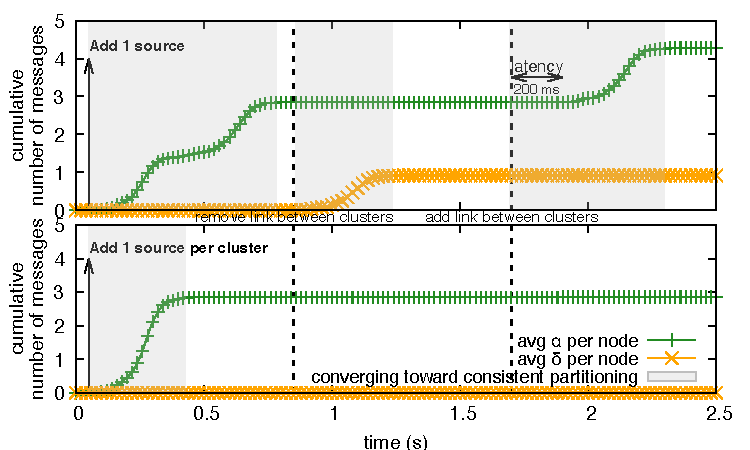
\includegraphics[width=\FIGSCALE\columnwidth]{img/as_cast_geant.pdf}
  \caption{\label{fig:geant}Partitioning overhead of 2
    clusters connected by a long distance link.}
\end{figure}


\subsection{Traffic containment}
\item [Objective:] Confirm that \NAME locks down the traffic of
  decentralized content indexing in dynamic
  inter-autonomous systems.
  
\item [Description:]

We build a network by duplicating the G{\'E}ANT
topology~\cite{knight2011internet} -- an infrastructure of 271 \nodes
spanning across Europe -- and we link these two clusters with a high
latency link: $200$ ms simulating cross-continental communications
such as Europe-America. The experiments comprise $2 \times 271 = 542$
\processes and we derive intra-cluster latency from their \processes'
geographic location.

\noindent We evaluate the traffic of \NAME by measuring the average
number of messages per \process over the experiments. In the first
experiment, at $50$~ms, only one \process becomes source, hence there
is only one partition for the whole distributed system. In the second
experiment, at $50$~ms, two \processes become sources, one per
cluster. Afterwards both scenarios are identical. At $850$~ms, we
remove the link between the two clusters. At $1.7$~s, we insert back
this link.

%% \begin{figure*}[t]
%%   \subfloat[\label{fig:nrens}Workload in 40 interconnected autonomous systems with
%%     1157 \processes~\cite{knight2011internet}.]{
%%     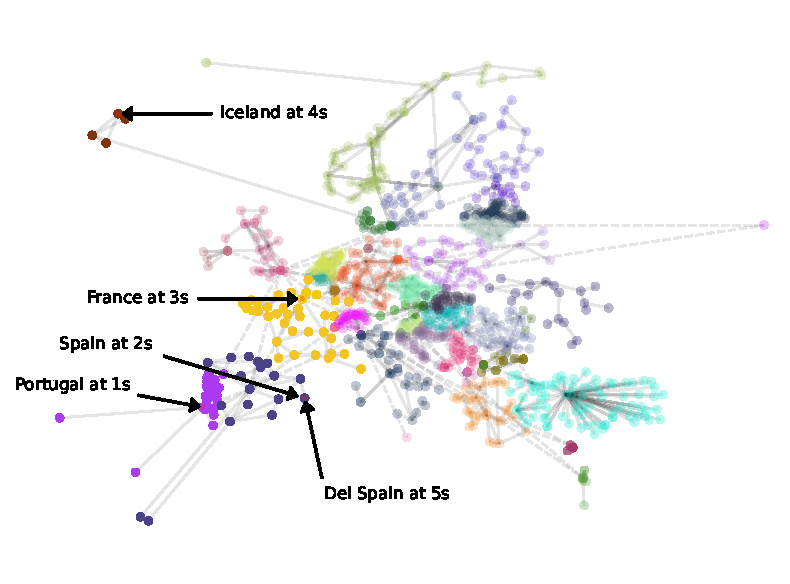
\includegraphics[width=\FIGSCALE\columnwidth]{img/europe-ases.pdf} 
%%   }
%%   \hspace{5pt}
%%   \subfloat[\label{fig:europe-ases}Traffic overhead and maintained indexes.]{
%%     \centering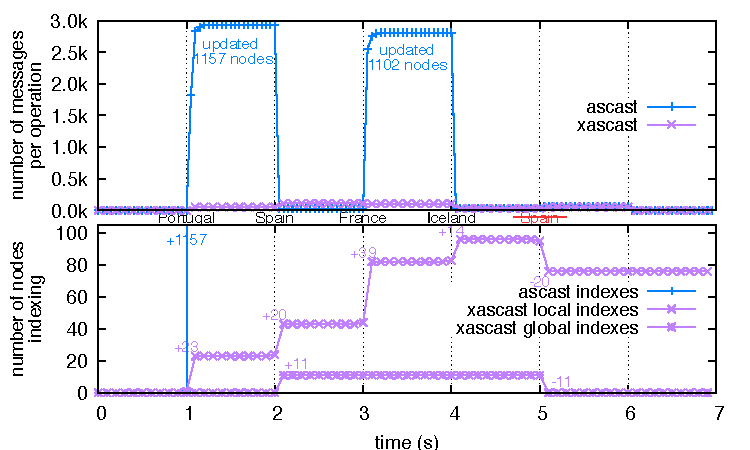
\includegraphics[width=\FIGSCALE\columnwidth]{img/europe_as_vs_xas.pdf}
%%   }
%%   \caption{Evaluation of \NAMEC for \emph{lazy} dynamic partitioning.}
%% \end{figure*}



\item [Results:]

Figure~\ref{fig:geant} shows the results of this experimentation. The
top part displays the results with one source while the bottom part
displays the results with one source per cluster.

\noindent Figure~\ref{fig:geant} confirms that concurrent
\texttt{Add}s may reach consistent partitioning faster. In particular,
the top part of Figure~\ref{fig:geant} depicts a slow down in traffic
around $300$ ms due to the high latency inter-continental link. The
first plateau shows the source's autonomous system acknowledging this
source, while the second shows the other autonomous system catching
up.  The inter-continental link is a bottleneck that does not exist
when each cluster has its own source.

\noindent Figure~\ref{fig:geant} highlights that \NAME operates well
even when \emph{physical} partitions appear. Indeed, the disconnection
of the inter-continental link existing between the two clusters
either leads to 
\begin{inparaenum}[(i)]
\item additional traffic when the \processes do not have any source in
  their cluster because \processes need to purge all indexes about the
  remote unreachable source until reaching consistent partitioning; or
  %\item an already consistent partitioning as \processes of each
  \item a status quo as \processes of each 
  cluster already target the source in their respective cluster.
\end{inparaenum}

\noindent Finally, Figure~\ref{fig:geant} shows that, when adding back the
inter-continental link, the two clusters can communicate again. In the
experiment involving one source for two clusters, it generates
traffic. After a $200$ milliseconds delay corresponding to the inter-continental link
latency, the cut off cluster starts to communicate $\alpha$ messages
again. Eventually, all \processes belong to the same
partition. However, in the experiment involving one source \emph{per}
cluster, the new link does not trigger noticeable traffic, for
\processes already know their closest source in their cluster.

\end{asparadesc}

%% \subsection{Cross autonomous systems}
%% \begin{asparadesc}
%% \item[Objective:] Highlight the shortcoming of \NAME in
%%   infrastructures composed of multiple autonomous systems and
%%     discuss an improvement called \underline{cross} \underline{\NAME}
%%     (\NAMEC). At coarse-grained, \NAMEC enables
%%     \emph{lazy} %\footnote{Laziness properties and \NAMEC would be
%%     %    further detailed in the  additional two pages available in the
%%     %    camera-ready version of the article.}
%%     dynamic partitioning by
%%     allowing AS' gateways to stop notifications when their respective
%%     network does not appear to have a source.
    
%%   \item[Description:] We build a network of networks comprising
%%     G{\'E}ANT along with the underlying European NRENs.
%%     Figure~\ref{fig:nrens} depicts the resulting infrastructure
%%     composed of 1157 \processes distributed in 40 interconnected
%%     autonomous systems spanning across
%%     Europe~\cite{knight2011internet}. \emph{Gateway} \processes (dark
%%     in the figure) link autonomous systems together, \eg a Lisbon
%%     \node links Portugal to Spain and United Kingdoms through a Madrid
%%     \node and a London \node respectively.

%%     \noindent Figure~\ref{fig:nrens} also depicts the operations
%%     executed during the 7 seconds simulation: at 1 second, a \node
%%     located in Lisbon, Portugal performs an \texttt{Add}, \ie Lisbon
%%     becomes a new source; at 2 seconds, a \node located in Palma de
%%     Majorque, Spain performs an \texttt{Add}; at 3 seconds, a \node
%%     located in Paris, France performs an \texttt{Add}; at 4 seconds, a
%%     \node located in Hvanneyri, Iceland performs an \texttt{Add};
%%     finally at 5 seconds, the \node in Spain performs a \texttt{Del},
%%     \ie the Spanish source is removed. We chose these sources to
%%     illustrate the limitations of \NAME while further motivating the
%%     importance of containing the traffic within relevant
%%     autonomous systems as proposed by \NAMEC.
    
%%     \noindent In \NAMEC, each
%%     \process maintains a \emph{local} index that corresponds to the
%%     best partition of its autonomous system, and a \emph{global}
%%     index that corresponds to the best partition cross autonomous
%%     systems, \ie adjacent autonomous systems that have at least one
%%     source.
    
%%     \noindent To compare \NAME against \NAMEC, we measure the number
%%     of messages transiting through the network for each operation, as
%%     well as the number of \processes that maintain an index (\ie that
%%     belong to a partition) over time.
    
%%   \item[Results:] Figure~\ref{fig:europe-ases} shows the
%%     results of this experiment. The top part highlights the cost of
%%     each partitioning protocol after each operation, while the bottom
%%     part provides the insight that explains these costs by displaying
%%     the number of indexes maintained by each protocol.

%%     \noindent Figure~\ref{fig:europe-ases} shows that Portugal's
%%     \texttt{Add} costs an order of magnitude more with \NAME compared
%%     to \NAMEC.  \NAME's messages propagate through all Europe, for
%%     \NAME regards Europe as a single network of 1157 \processes while
%%     \NAMEC's messages propagate through Portugal's network of 23
%%     \processes only.
%%     % 
%%     \noindent  Spain's
%%     \texttt{Add} costs slightly more with \NAMEC compared to \NAME.  A
%%     gateway in Madrid links Portugal to Spain and the rest of
%%     Europe. Since Lisbon is closer to Madrid than Palma de Majorque
%%     is, only 11 \processes in Spain actually need to receive and
%%     deliver the new notification, which explains the small overhead of this
%%     operation with \NAME. Using \NAMEC, the overhead is slightly
%%     higher since
%%     \begin{inparaenum}[(i)]
%%     \item the 20 \processes of Spain's network need to receive and
%%       deliver the new notification, \emph{and}
%%     \item Madrid's gateway echoes Lisbon's notification as soon as it
%%       receives Palma's notification to 11 \processes.
%%     \end{inparaenum}

%%     \noindent Figure~\ref{fig:europe-ases} also highlights the worst
%%     case scenario of \NAME: the cost of France's \texttt{Add} is close
%%     to that of Portugal's \texttt{Add} since it updates the whole
%%     Europe excluding Portugal and Spain. Contrarily, \NAMEC only
%%     updates France's 39 \processes.

%%     \noindent The last \texttt{Add} operation in Iceland has similar
%%     cost for \NAME and \NAMEC. Indeed, they both update Iceland, and
%%     when the notifications reach Copenhagen in Danemark, they stop
%%     either because France's notifications are closer (\NAME) or the
%%     Danish network does not have any source (\NAMEC).

%%     \noindent Finally, Figure~\ref{fig:europe-ases} shows that
%%     Spain's \texttt{Del} have similar cost for \NAME and
%%     \NAMEC. Nevertheless, the trade-off is different: \NAME's overhead
%%     comes from the 11 \nodes that need to acknowledge staleness and
%%     deliver the echos from Portugal; \NAMEC's overhead comes from the
%%     20 \nodes that need to acknowledge staleness. Using \NAMEC,
%%     Spain's network does not propagate echos since it does not have
%%     any source anymore.

%% \end{asparadesc}

%% \begin{asparadesc}
%%   \item[\TODO{Overall:}] this experimentation empirically demonstrates the
%%     benefits of \NAME in the context of geo-distributed
%%     infrastructures, e.g., inter-connected autonomous systems where
%%     \processes and communications links may be added and removed at
%%     any time. \NAME coupled with replication strategies designed for
%%     Edge infrastructures would allow locking down the traffic of
%%     replica indexing, while providing every \process with quick access
%%     to replicated content.
%% \end{asparadesc}

\begin{asparadesc}
  \item[Overall,] these experiments highlight the scalability of \NAME
    and \NAMEC in dynamic networks such as Edge infrastructures. Next
    Section reviews state-of-the-art approaches that can index content
    in geo-distributed infrastructures.
\end{asparadesc}


%% Next Section reviews state-of-the-art approaches for content indexing
%%  in geo-distributed infrastructures and explains their shortcomings.

%%% Local Variables: 
%%% mode: latex
%%% TeX-master: "../paper"
%%% ispell-local-dictionary: "english"
%%% End: 
